\documentclass{beamer}
\usepackage[T1]{fontenc}
%\usepackage{arevtext,arevmath}
%\usepackage{ccfonts} 
\usepackage[utf8]{inputenc}
%\usepackage[italian]{babel}
\usetheme{Rochester}
\usefonttheme[onlymath]{serif}
\usepackage{diffcoeff}
\usepackage{graphicx}
\usepackage{bm}
\usepackage{amsmath}
\usepackage{amssymb}
\usepackage{wrapfig}
\usepackage{amsfonts}
\usepackage{amsthm}
\usepackage{amscd}
\usepackage{multicol}
\newenvironment{sistema}%
{\left\lbrace\begin{array}{@{}l@{}}}%
{\end{array}\right.}

\title{Gene Regulatory Networks for Cellular Differentiation - a Random Boolean Network Approach}%\author{Riccardo Scheda \\ \flushleft{Relatore: Prof. Armando Bazzani}}
\institute[]{Applied Physics \\ University of Bologna}
\author{\Large{Riccardo Scheda}}
\date{May 2020}


\begin{document}

\begin{frame}
\maketitle
\end{frame}


\begin{frame}
\frametitle{Introduction}
\centering
Cellular Differentiation
\begin{figure}
\centering
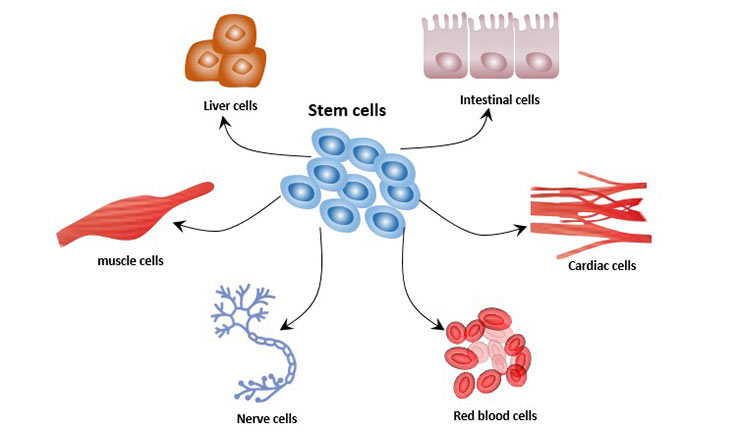
\includegraphics[scale=0.4]{celldiff.jpg}
\end{figure}
\end{frame}

\begin{frame}
\frametitle{Fitness Landscape}
\centering

\begin{figure}
\centering
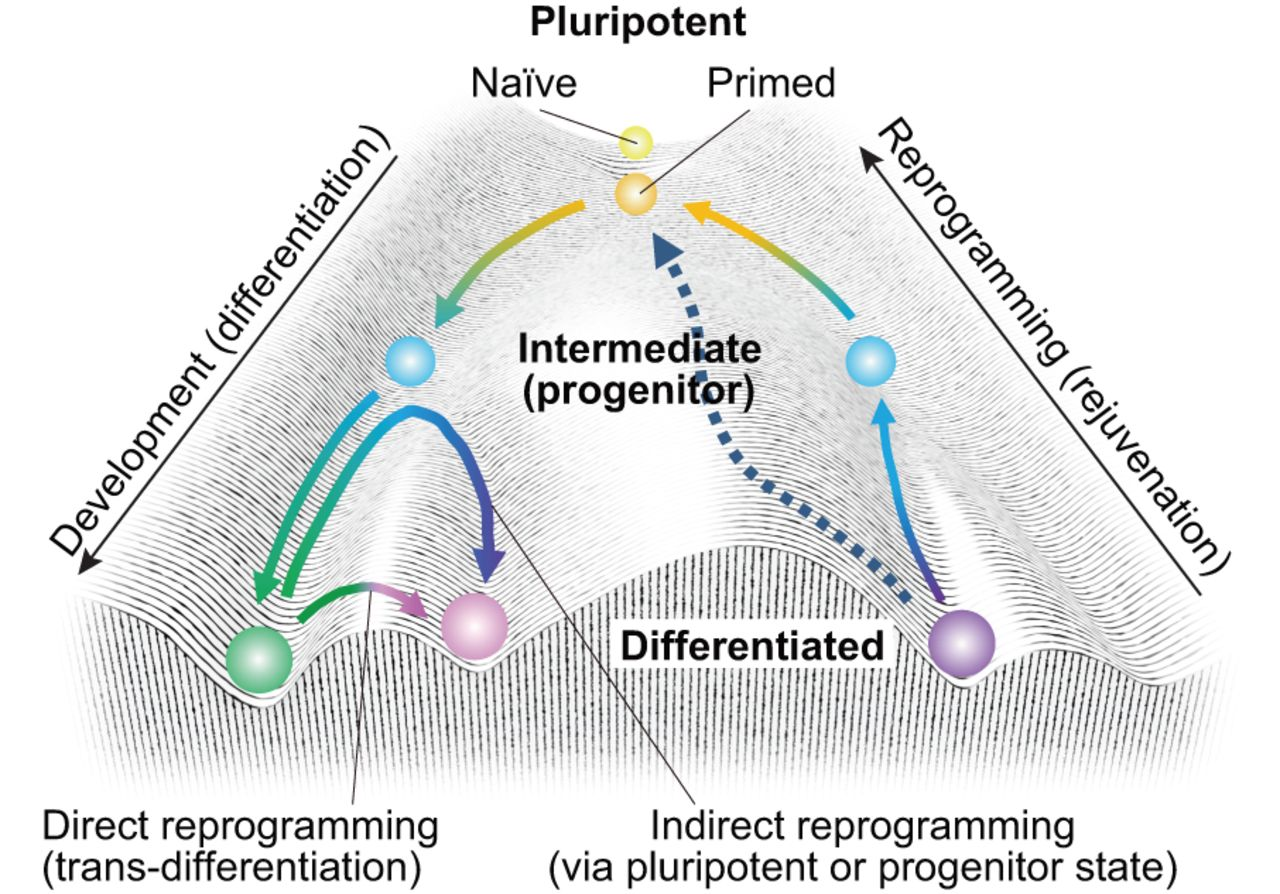
\includegraphics[scale=0.8]{landscape.jpg}
\end{figure}
\end{frame}

\begin{frame}
\frametitle{Gene Regulatory Networks}
Cellular differentiation and other mechanisms in cell dynamics are governed by the gene regulatory networks (GRN)

\begin{figure}
\centering
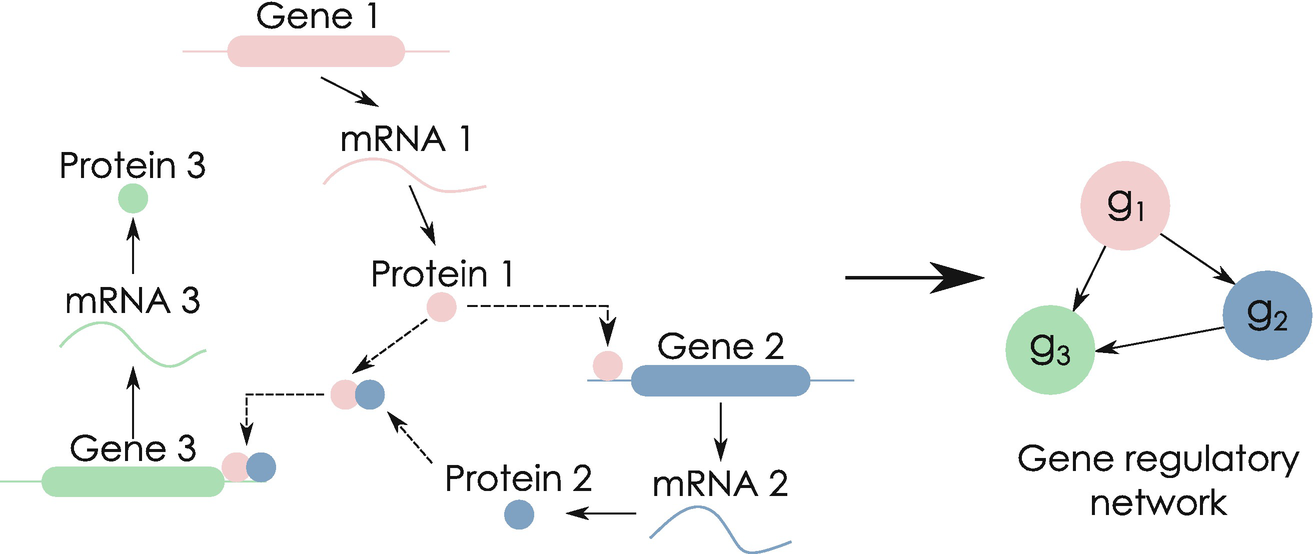
\includegraphics[scale=1]{GRN.png}
\end{figure}
\end{frame}


\begin{frame}
\frametitle{Mutation}

Studies confirmed that during the process of GRN we can have mutations in the networks which cause the birth of cancer cells
\centering

\begin{figure}
\centering
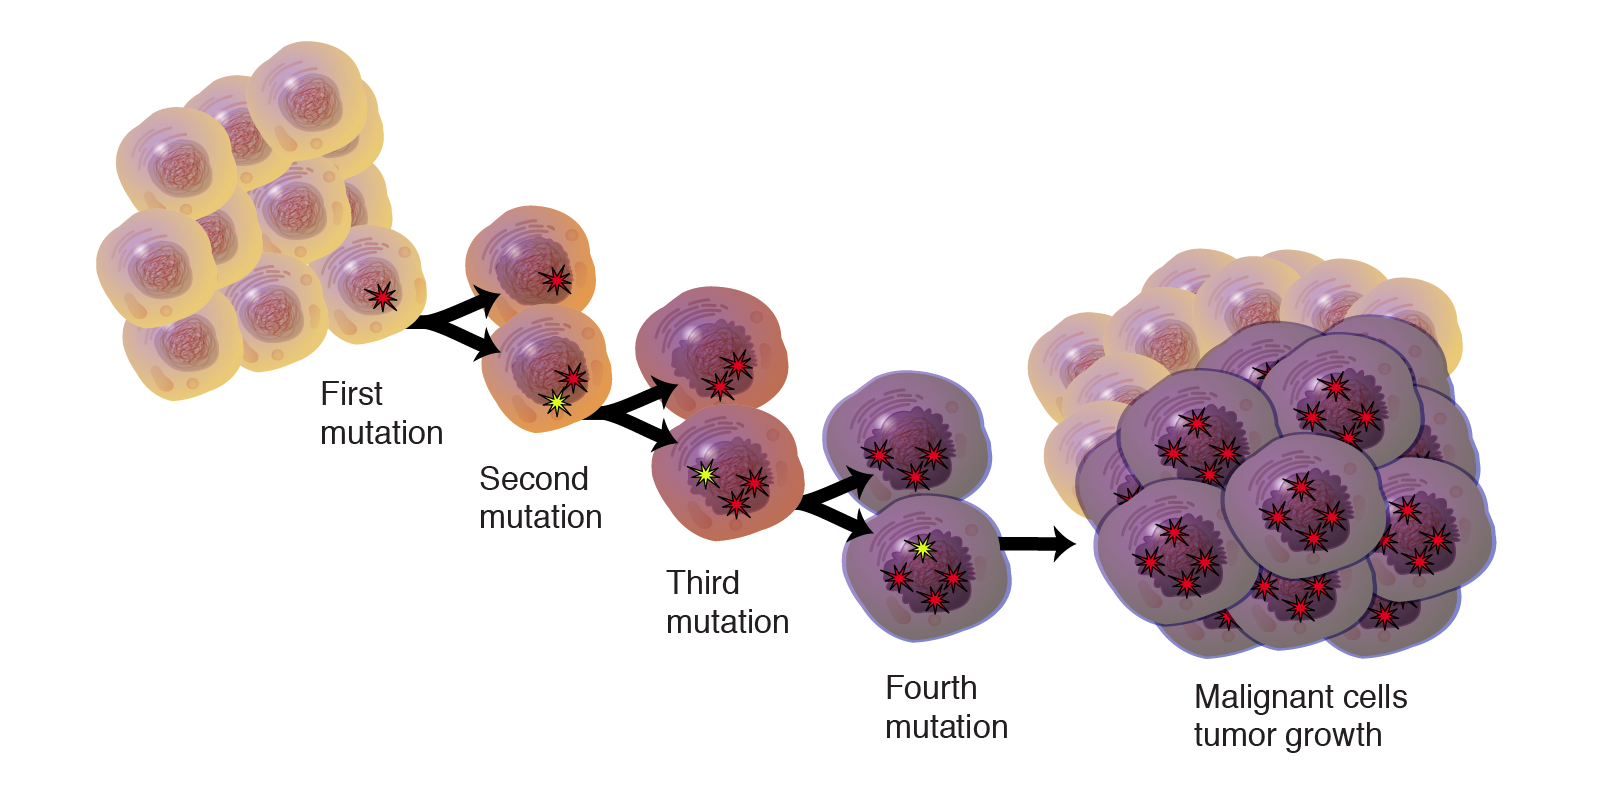
\includegraphics[scale=0.2]{mutation.jpg}
\end{figure}
\end{frame}


\begin{frame}
\frametitle{Modelling GRN - Random Boolean Networks}
Stuart Kauffman proposed to model GRN using Random Boolean Networks (RBN)
which are networks in which each gene is a node in a directed graph and can be "on" or "off", so we have that each node $\sigma_i$ can have values 0 or 1.

\begin{figure}
\centering
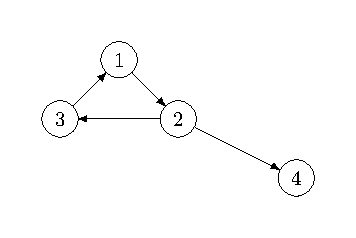
\includegraphics{figurenetworks2.pdf}
\end{figure}
\end{frame}



\begin{frame}
\frametitle{RBN Dynamics}
The evolution of the state of each node $\sigma_i(t)$ is given by a Boolean function $\Lambda_i(\sigma_{i_1},...,\sigma_{i_k})$ of K parameters, which are the incoming links from the other nodes in the network:


$$
\sigma_i(t+1) = \Lambda_i(\sigma_{i_1}(t),...\sigma_{i_k}(t))
$$
\begin{figure}
\centering
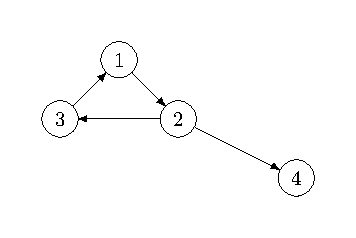
\includegraphics{figurenetworks2.pdf}
\end{figure}
\end{frame}

\begin{frame}
\frametitle{RBN Dynamics}
\begin{figure}
\centering
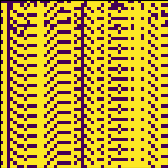
\includegraphics{rbn.png}
\caption{Example of a RBN with $N=50$ and $K=1$. }
\end{figure}
\end{frame}


\begin{frame}
\frametitle{State space}
For example we can consider an evolution of the network with number of nodes $N=4$ in this form:
$$
1111 \to 0011 \to 0100 \to 1111
$$

If we interpret the bit sequence characterizing the state of the network as a number in binary notation, the sequence of states can also be
written as

$$
15 \to 3 \to 4 \to 15
$$
 Since
the update rule is deterministic, the same state must always be followed by
the same next state:

$$
15 \to 3 \to 4 \to 15 \to 3 \to 4 \to 15 \to \dots
$$
So starting from some initial state, the network performs a trajectory in state space and eventually arrives on a periodic sequence, called \emph{attractor}
\end{frame}






\begin{frame}
\frametitle{Attractors}
Now, we can represent the different configurations in a network:
\begin{figure}
\centering
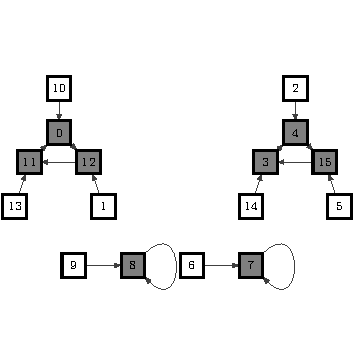
\includegraphics{fg3.pdf}
\end{figure}
\end{frame}



\begin{frame}
\frametitle{Perturbations}


Flipping a bit:
$$
1100 \to 1110
$$




\begin{figure}[h]
\centering
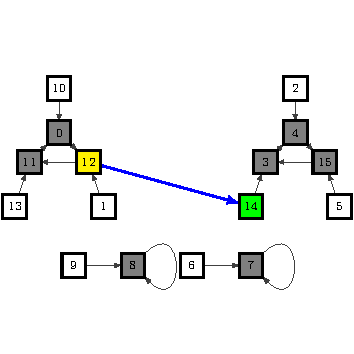
\includegraphics[scale=0.8]{fg4.pdf}
\caption{Jump from one attractor to another one in the state space}
\label{fig:rb4}
\end{figure}

\end{frame}



\begin{frame}
\frametitle{Attractors}
We can construct the network of the attractors, where the links connect different attractor after a perturbation:
\begin{figure}
\centering
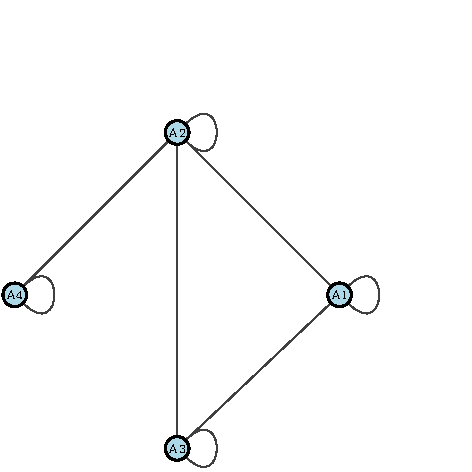
\includegraphics[scale=0.6]{fg5.pdf}
\caption{Network of attractors of a RBN}
\end{figure}
\end{frame}


\begin{frame}
\frametitle{Stochastic process}
\begin{figure}
\centering
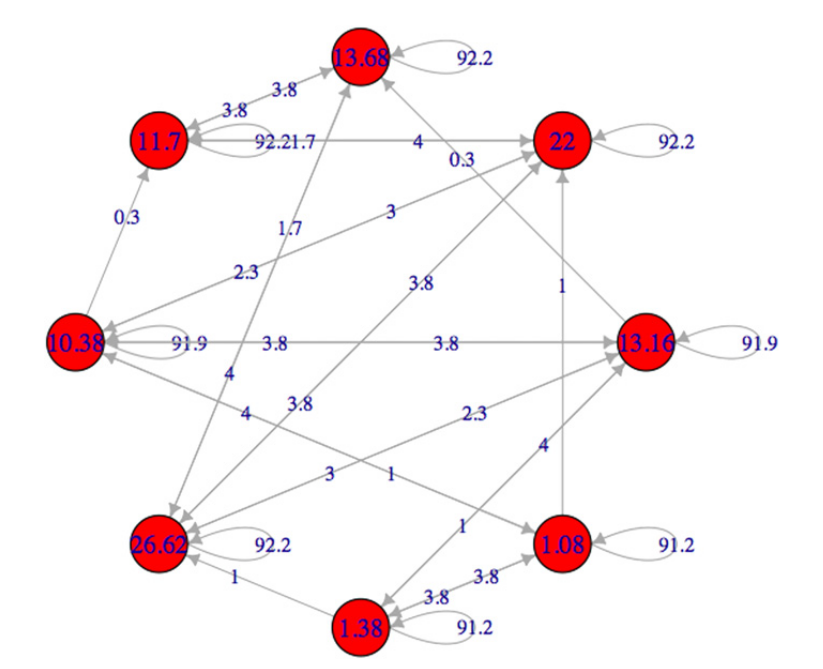
\includegraphics[scale=0.2]{matrix.png}

\end{figure}
From the network of the attractors, we can analyze the different frequencies of transtion between an attractor from another one, and build a stochastic process.
\end{frame}



\begin{frame}
\frametitle{Conclusions}
From this model, we can associate different attractors to different type of cells, and in particular cancer cell can be considered as little attractors in the network.


So the aim of this thesis work is to build a stochastic process and a random walk on a network of attractors of a RBN.



\end{frame}




\end{document}


Since we are talking about gene networks for cell differentiation,
we can consider attractors in the state space as gene regulatory networks of different cells, where different attractors represent cells of different type, and where for example cancer cells lay in one specific attractor.
Now, if we suppose that different cell types lay in different attractors, we can suppose that the jump from an attractor to one other is given by a perturbation in the binary sequence of the genes.
So for example we take the previos network, and consider that we are in the state $12$ of the first attractor:

And suddenly we change the state of the third node from $0$ to $1$:

We change the system to have the state $14$ and so we jump into the second attractor:

